% Hình 5.3: So sánh Soft IoU trung bình của 7 mô hình trên PH2 (trái) và GlaS 2015 (phải)
% Số liệu 5-fold từ báo cáo. Vẽ bằng pgfplots (không lấy từ evaluate.py).
% Xanh = baseline cổ điển; cam = QuNet (mốc lượng tử QuFeX); tím = HQMoSS-Net (đề xuất).
\documentclass[border=6pt]{standalone}
\usepackage[utf8]{vietnam}
\usepackage{amsmath}
\usepackage{xcolor}
\usepackage{pgfplots}
\pgfplotsset{compat=1.17}
\usepgfplotslibrary{groupplots}
\definecolor{cvblue}{HTML}{5B86B0}
\definecolor{qamber}{HTML}{E39A3B}
\definecolor{qpurple}{HTML}{7E57C2}
\definecolor{inkdark}{HTML}{23272E}
\begin{document}
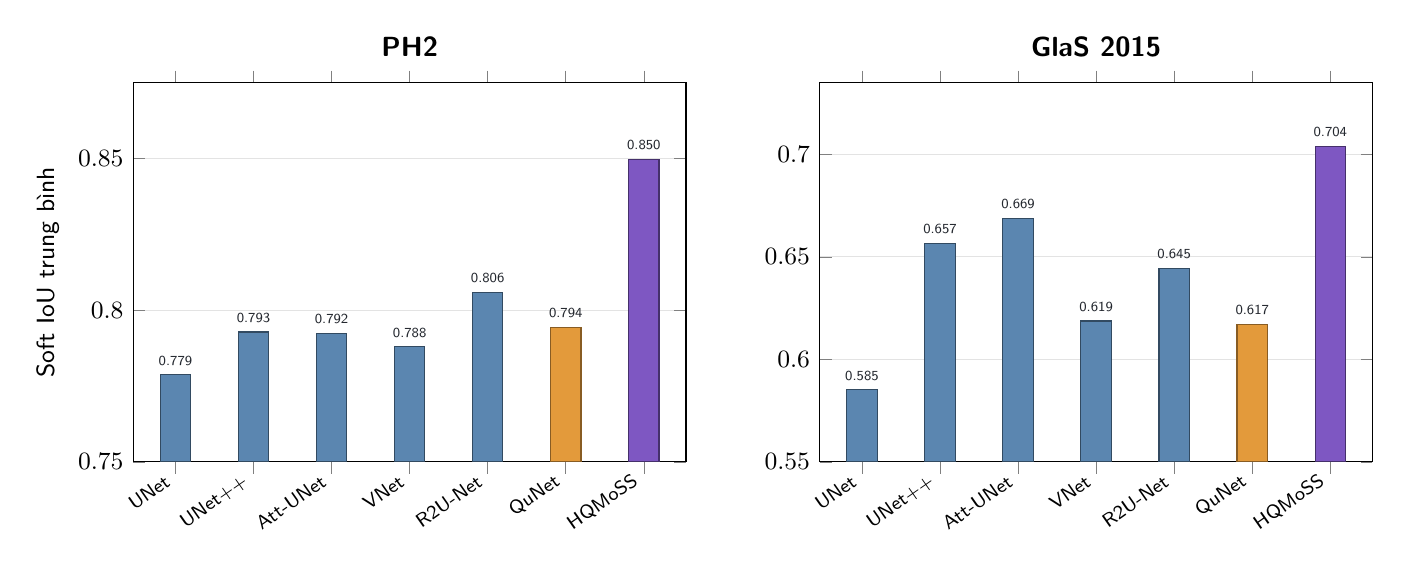
\begin{tikzpicture}
\begin{groupplot}[
  group style={group size=2 by 1, horizontal sep=1.7cm},
  width=8.6cm, height=6.4cm,
  ymajorgrids, grid style={gray!22},
  tick label style={font=\sffamily\small},
  label style={font=\sffamily\small},
  title style={font=\sffamily\bfseries},
  nodes near coords, point meta=explicit symbolic,
  every node near coord/.append style={font=\sffamily\tiny, anchor=south, text=inkdark},
  xtick={1,2,3,4,5,6,7},
  xticklabels={UNet, UNet++, Att-UNet, VNet, R2U-Net, QuNet, HQMoSS},
  x tick label style={rotate=35, anchor=east, font=\sffamily\scriptsize},
  enlarge x limits=0.09,
]
\nextgroupplot[ybar, bar width=11pt, title={PH2}, ylabel={Soft IoU trung bình}, ymin=0.75, ymax=0.875]
\addplot[fill=cvblue, draw=cvblue!55!black, bar shift=0pt] coordinates
  {(1,0.7787)[0.779] (2,0.7928)[0.793] (3,0.7923)[0.792] (4,0.7879)[0.788] (5,0.8058)[0.806]};
\addplot[fill=qamber, draw=qamber!60!black, bar shift=0pt] coordinates
  {(6,0.7942)[0.794]};
\addplot[fill=qpurple, draw=qpurple!55!black, bar shift=0pt] coordinates
  {(7,0.8497)[0.850]};
\nextgroupplot[ybar, bar width=11pt, title={GlaS 2015}, ymin=0.55, ymax=0.735]
\addplot[fill=cvblue, draw=cvblue!55!black, bar shift=0pt] coordinates
  {(1,0.5851)[0.585] (2,0.6567)[0.657] (3,0.6689)[0.669] (4,0.6187)[0.619] (5,0.6445)[0.645]};
\addplot[fill=qamber, draw=qamber!60!black, bar shift=0pt] coordinates
  {(6,0.6171)[0.617]};
\addplot[fill=qpurple, draw=qpurple!55!black, bar shift=0pt] coordinates
  {(7,0.7038)[0.704]};
\end{groupplot}
\end{tikzpicture}
\end{document}
